\documentclass[tikz,border=10pt]{standalone}
\usepackage[utf8]{inputenc}
\usepackage[T5]{fontenc}
\usepackage{xcolor}
\usepackage{amsmath,amssymb,amsfonts}
\usepackage{helvet}
\renewcommand{\familydefault}{\sfdefault}

\usetikzlibrary{shapes.geometric,arrows.meta,positioning,fit,
                backgrounds,calc,decorations.pathreplacing,patterns}

% ── Colours ──────────────────────────────────────────────────────────────────
\definecolor{C_slate}{RGB}{71,85,105}     \definecolor{C_blue}{RGB}{59,130,246}
\definecolor{C_indigo}{RGB}{99,102,241}   \definecolor{C_amber}{RGB}{245,158,11}
\definecolor{C_rose}{RGB}{244,63,94}      \definecolor{C_sky}{RGB}{14,165,233}
\definecolor{C_bglight}{RGB}{248,250,252} \definecolor{C_bgmid}{RGB}{241,245,249}
\definecolor{C_emerald}{RGB}{16,185,129}  \definecolor{negcol}{RGB}{16,185,129}
\definecolor{C_violet}{RGB}{139,92,246}   \definecolor{C_fuchsia}{RGB}{200,50,220}
\definecolor{headcol}{RGB}{30,41,59}

\begin{document}

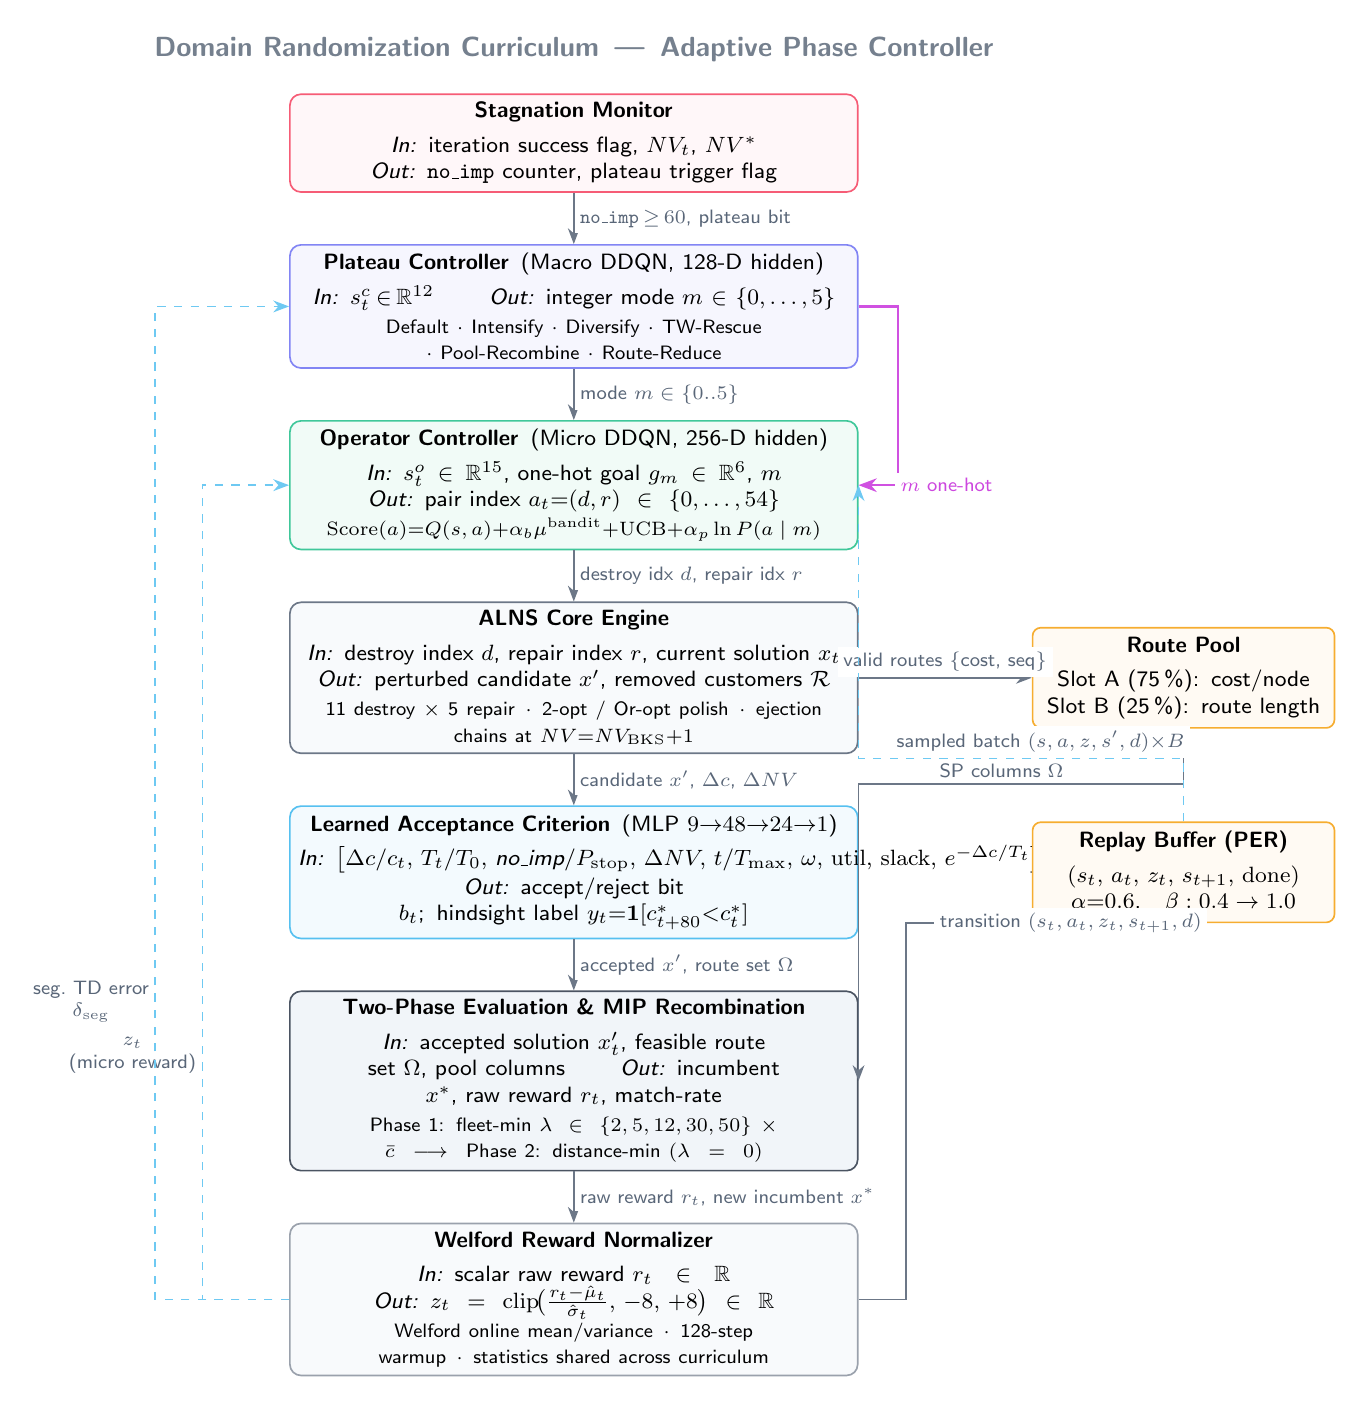
\begin{tikzpicture}[
    font=\sffamily\footnotesize, >=Stealth,
    node distance=0.65cm and 2.5cm,
    %% ── Block styles ──────────────────────────────────────────────
    det/.style={rectangle, rounded corners=4pt, semithick, align=center,
                minimum width=7.2cm, minimum height=1.0cm, text width=7.0cm, inner sep=3pt},
    mon/.style ={det, draw=C_rose!85,    fill=C_rose!4},
    mac/.style ={det, draw=C_indigo!80,  fill=C_indigo!6},
    mic/.style ={det, draw=C_emerald!80, fill=C_emerald!6},
    alns/.style={det, draw=C_slate!80,   fill=C_bglight},
    lac/.style ={det, draw=C_sky!70,     fill=C_sky!5},
    eval/.style={det, draw=headcol!80,   fill=C_bgmid},
    norm/.style={det, draw=C_slate!55,   fill=C_bglight},
    mem/.style ={rectangle, rounded corners=3pt, semithick, align=center,
                 minimum width=3.8cm, minimum height=1.0cm, text width=3.6cm,
                 draw=C_amber!85, fill=C_amber!5, font=\sffamily\footnotesize},
    %% ── Arrow styles ──────────────────────────────────────────────
    flow/.style={->, semithick, draw=C_slate!80},
    back/.style={->, dashed, semithick, draw=C_sky!60},
    goal/.style={->, thick, draw=C_fuchsia!85},
    lbl/.style={font=\sffamily\scriptsize, fill=white, inner sep=2pt,
                text=C_slate!90, align=center}
]

%% ── Main pipeline (center column) ──────────────────────────────────────────
\node[mon] (M) {%
  \textbf{Stagnation Monitor}\\[3pt]
  \textit{In:}\enspace iteration success flag, $NV_t$, $NV^*$
  \qquad
  \textit{Out:}\enspace \texttt{no\_imp} counter, plateau trigger flag};

\node[mac, below=of M] (PC) {%
  \textbf{Plateau Controller}\enspace(Macro DDQN, 128-D hidden)\\[3pt]
  \textit{In:}\enspace $s_t^c\!\in\!\mathbb{R}^{12}$
  \qquad
  \textit{Out:}\enspace integer mode $m\in\{0,\ldots,5\}$\\[1pt]
  \scriptsize Default $\cdot$ Intensify $\cdot$ Diversify $\cdot$
  \mbox{TW-Rescue} $\cdot$ Pool-Recombine $\cdot$ Route-Reduce};

\node[mic, below=of PC] (OC) {%
  \textbf{Operator Controller}\enspace(Micro DDQN, 256-D hidden)\\[3pt]
  \textit{In:}\enspace $s_t^o\!\in\!\mathbb{R}^{15}$,\ one-hot goal $g_m\!\in\!\mathbb{R}^6$,\ $m$
  \qquad
  \textit{Out:}\enspace pair index $a_t{=}(d,r)\in\{0,\ldots,54\}$\\[1pt]
  \scriptsize $\mathrm{Score}(a){=}Q(s,a){+}\alpha_b\mu^{\mathrm{bandit}}{+}\mathrm{UCB}{+}\alpha_p\ln P(a\!\mid\!m)$};

\node[alns, below=of OC] (AE) {%
  \textbf{ALNS Core Engine}\\[3pt]
  \textit{In:}\enspace destroy index $d$, repair index $r$, current solution $x_t$
  \qquad
  \textit{Out:}\enspace perturbed candidate $x'$, removed customers $\mathcal{R}$\\[1pt]
  \scriptsize 11 destroy $\times$ 5 repair\enspace$\cdot$\enspace
  \mbox{2-opt / Or-opt polish}\enspace$\cdot$\enspace ejection chains at $NV{=}NV_{\mathrm{BKS}}{+}1$};

\node[lac, below=of AE] (LA) {%
  \textbf{Learned Acceptance Criterion}\enspace(MLP $9{\to}48{\to}24{\to}1$)\\[3pt]
  \textit{In:}\enspace $\bigl[\Delta c/c_t,\, T_t/T_0,\, \textit{no\_imp}/P_{\mathrm{stop}},\, \Delta NV,\, t/T_{\max},\, \omega,\, \mathrm{util},\, \mathrm{slack},\, e^{-\Delta c/T_t}\bigr]$\\[1pt]
  \textit{Out:}\enspace accept/reject bit $b_t$;\enspace
    hindsight label $y_t{=}\mathbf{1}[c^*_{t+80}{<}c^*_t]$};

\node[eval, below=of LA] (EV) {%
  \textbf{Two-Phase Evaluation \& MIP Recombination}\\[3pt]
  \textit{In:}\enspace accepted solution $x_t'$, feasible route set $\Omega$, pool columns
  \qquad
  \textit{Out:}\enspace incumbent $x^*$, raw reward $r_t$, match-rate\\[1pt]
  \scriptsize \mbox{Phase 1: fleet-min} $\lambda\in\{2,5,12,30,50\}\times\bar{c} \longrightarrow \mbox{Phase 2: distance-min } (\lambda=0)$};

\node[norm, below=of EV] (WN) {%
  \textbf{Welford Reward Normalizer}\\[3pt]
  \textit{In:}\enspace scalar raw reward $r_t\in\mathbb{R}$
  \qquad
  \textit{Out:}\enspace $z_t=\mathrm{clip}\!\bigl(\tfrac{r_t-\hat{\mu}_t}{\hat{\sigma}_t},\,-8,\,+8\bigr)\in\mathbb{R}$\\[1pt]
  \scriptsize Welford online mean/variance\enspace$\cdot$\enspace
  128-step warmup\enspace$\cdot$\enspace statistics shared across curriculum};

%% ── Side memory nodes ───────────────────────────────────────────────────────
\node[mem, right=2.2cm of AE] (RP) {%
  \textbf{Route Pool}\\[3pt]
  Slot A (75\,\%): cost/node\\
  Slot B (25\,\%): route length};

\node[mem, right=2.2cm of LA] (PER) {%
  \textbf{Replay Buffer (PER)}\\[3pt]
  $(s_t,\,a_t,\,z_t,\,s_{t+1},\,\mathrm{done})$\\
  $\alpha{=}0.6$,\quad$\beta\!:\!0.4\!\to\!1.0$};

%% ── Forward flows (labeled with actual data payload) ────────────────────────
\draw[flow] (M)  -- node[lbl, right]
  {\texttt{no\_imp}$\,{\ge}\,60$, plateau bit} (PC);

\draw[flow] (PC) -- node[lbl, right]
  {mode $m\in\{0..5\}$} (OC);

\draw[flow] (OC) -- node[lbl, right]
  {destroy idx $d$,\ repair idx $r$} (AE);

\draw[flow] (AE) -- node[lbl, right]
  {candidate $x'$,\ $\Delta c$,\ $\Delta NV$} (LA);

\draw[flow] (LA) -- node[lbl, right]
  {accepted $x'$,\ route set $\Omega$} (EV);

\draw[flow] (EV) -- node[lbl, right]
  {raw reward $r_t$,\ new incumbent $x^*$} (WN);

%% ── Side flows ──────────────────────────────────────────────────────────────
\draw[flow] (AE.east)  -- node[lbl, above]
  {valid routes $\{$cost, seq$\}$} (RP.west);

\draw[flow] (RP.south) -- ++(0,-0.7) -|
  node[lbl, pos=0.28, above] {SP columns $\Omega$} (EV.east);

\draw[flow] (WN.east)  -- ++(0.6,0) |-
  node[lbl, pos=0.55, right]
  {transition $(s_t,a_t,z_t,s_{t+1},d)$} (PER.south);

%% ── Reward feedback ─────────────────────────────────────────────────────────
\draw[back] (PER.north) -- ++(0,0.8) -|
  node[lbl, pos=0.22, above]
  {sampled batch $(s,a,z,s',d){\times}B$} (OC.east);

\draw[back] (WN.west) -- ++(-1.1,0) |-
  node[lbl, pos=0.15, left]
  {$z_t$\\ (micro reward)} (OC.west);

\draw[back] (WN.west) -- ++(-1.7,0) |-
  node[lbl, pos=0.15, left]
  {seg.\ TD error\\ $\delta_{\mathrm{seg}}$} (PC.west);

%% ── Goal-conditioning vector ────────────────────────────────────────────────
\draw[goal] (PC.east) -- ++(0.5,0) |-
  node[lbl,pos=0.55,right,text=C_fuchsia!90]{$m$ one-hot} (OC.east);

%% ── Section title ───────────────────────────────────────────────────────────
\node[above=8pt of M, font=\sffamily\bfseries, text=C_slate!75]
  {Domain Randomization Curriculum\enspace---\enspace Adaptive Phase Controller};

\end{tikzpicture}

\end{document}
